\documentclass{beamer}

\usepackage[utf8]{inputenc}
\usepackage{default}
\usepackage{hyperref}
\usepackage{graphicx}
\usepackage{amsmath}
\usepackage{subcaption}
\usepackage{dsfont}

\usetheme{Warsaw}

\title{Implémentation du PageRank avec MPI}
\author{Ayaz \textsc{Badouraly}}
\date{13 avril 2016}
\institute{École Centrale Paris}

%\addtobeamertemplate{footline}{\insertframenumber/\inserttotalframenumber}

\beamertemplatetransparentcovered
\setbeamertemplate{footline}{
\leavevmode%
\hbox{\hspace*{-0.06cm}

\setbeamercolor{author in head/foot}{fg=white,bg=black}
\begin{beamercolorbox}[wd=.2\paperwidth,ht=2.25ex,dp=1ex,center]{author in head/foot}%
	\usebeamerfont{author in head/foot}\insertshortauthor%~~(\insertshortinstitute)
\end{beamercolorbox}%
\setbeamercolor{section in head/foot}{fg=white,bg=blue}
\begin{beamercolorbox}[wd=.7\paperwidth,ht=2.25ex,dp=1ex,center]{section in head/foot}%
	\usebeamerfont{section in head/foot}\insertshorttitle
\end{beamercolorbox}%
\begin{beamercolorbox}[wd=.1\paperwidth,ht=2.25ex,dp=1ex,center]{author in head/foot}%
	\usebeamerfont{author in head/foot}\insertframenumber{} / \inserttotalframenumber\hspace*{2ex}
\end{beamercolorbox}}%
\vskip0pt%
}

\begin{document}

  \AtBeginSection[]
  {
    \begin{frame}<beamer>
      \frametitle{Plan}
      \tableofcontents[currentsection]%,currentsubsection]
    \end{frame}
  }

  \AtBeginSubsection[]
  {
    \begin{frame}<beamer>
      \frametitle{Plan}
      \tableofcontents[currentsection,currentsubsection]
    \end{frame}
  }

  \begin{frame}%{Introduction}
    \titlepage
  \end{frame}
  
  
  \begin{frame}<beamer>
    \frametitle{Plan}
    \tableofcontents%[currentsection]%,currentsubsection]
  \end{frame}

  \section{Introduction}

    \begin{frame}
      \begin{block}{Cadre historique : 1998, invention du \textit{pagerank}}
        \bigskip
        \begin{figure}
          \begin{subfigure}{.48\textwidth}
            \centering
            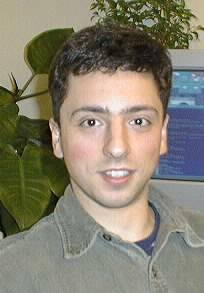
\includegraphics[height=4cm]{sergey_brin.jpg}
            \caption*{Sergey \textsc{Brin}}
          \end{subfigure}
          \begin{subfigure}{.48\textwidth}
            \centering
            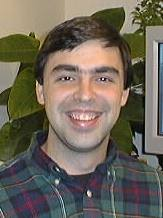
\includegraphics[height=4cm]{larry_page.jpg}
            \caption*{Lawrence \textsc{Page}}
          \end{subfigure}
        \end{figure}
        \medskip
      \end{block}
    \end{frame}
    
    \begin{frame}
      \begin{block}{Problématique}
        \bigskip
        \begin{itemize}
          \item En pratique : jeux de données énormes
          \medskip
          \pause \item Solution : librairie \texttt{MPI}
        \end{itemize}
        \bigskip
      \end{block}
    \end{frame}
  
  \section{Algorithme du pagerank}
  
    \begin{frame}
      \begin{block}{Modélisation de la navigation du surfeur}
        \bigskip
        \begin{itemize}
          \item $A$ : le surfeur clique sur un lien externe de sa page courante
          \medskip
          \pause \item $D$ : le surfeur arrive sur une page sans lien externe
          \medskip
          \pause \item $E$ : le surfeur change de page au hasard
        \end{itemize}
        \bigskip
      \end{block}
    \end{frame}
    
    \begin{frame}
      \begin{block}{Modélisation du web}
        \bigskip
        $$ M = dA + dD + (1-d)E $$
        
        où $d$ est le \textit{damping factor}
        \bigskip
      \end{block}
    \end{frame}
    
    \begin{frame}
      \begin{alertblock}{Définition du pagerank}
        \bigskip
        $$ Mp = p $$
        \medskip
      \end{alertblock}
      
      \begin{alertblock}{Algorithme du pagerank}
        \bigskip
        $$
          \left\{
            \begin{array}{llcl}
              & p^0 & = & \begin{pmatrix}
                \frac{1}{\text{dim}(M)} \\
                \vdots \\
                \frac{1}{\text{dim}(M)}
              \end{pmatrix}\\
            \forall n \in \mathds{N} : & p^{n+1} & = & M p^n 
            \end{array}
          \right.
        $$
        \medskip
      \end{alertblock}
    \end{frame}
  
  \section{Implémentation}
  
  \subsection{Les structures de données}
  
  \begin{frame}{Les vecteurs}
    \begin{minipage}[c]{.30\linewidth}
      \begin{exampleblock}{Vecteur mathématique}
        \bigskip
        $$
        \begin{pmatrix}
          1 \\
          2 \\
          3 \\
          4 \\
          5 \\
          6
        \end{pmatrix}
        $$
        \bigskip
      \end{exampleblock}
    \end{minipage} \hfill
    \begin{minipage}[c]{.60\linewidth}
      \begin{exampleblock}{Vecteur informatique}
        \vspace{1.3cm}
        $$
        \left\{
          \begin{array}{lcl}
            \texttt{dim} & = & 6 \\
            \texttt{vector} & = & [1;2;3;4;5;6]
          \end{array}
        \right.
        $$
        \vspace{1.3cm}
      \end{exampleblock}
    \end{minipage}
  \end{frame}
  
  \begin{frame}{Les matrices COO}
    \begin{minipage}[c]{.30\linewidth}
      \begin{exampleblock}{Matrice mathématique}
        \bigskip
        $$
        \begin{pmatrix}
          1 & 2 & 3 & 0 & 0 \\
          0 & 0 & 0 & 4 & 5 \\
          0 & 0 & 0 & 6 & 7 \\
          0 & 0 & 0 & 0 & 8 \\
          0 & 0 & 0 & 9 & 0
        \end{pmatrix}
        $$
        \bigskip
      \end{exampleblock}
    \end{minipage} \hfill
    \begin{minipage}[c]{.60\linewidth}
      \begin{exampleblock}{Matrice informatique}
        \vspace{0.9cm}
        $$
        \left\{
          \begin{array}{lcl}
            \texttt{nnz} & = & 9 \\
            \texttt{rows} & = & [0;0;0;1;1;2;2;3;4] \\
            \texttt{cols} & = & [0;1;2;3;4;3;4;4;3] \\
            \texttt{values} & = & [1;2;3;4;5;6;7;8;9]
          \end{array}
        \right.
        $$
        \vspace{0.9cm}
      \end{exampleblock}
    \end{minipage}
  \end{frame}
  
  \begin{frame}{Exemples de matrices creuses}
    \only<1>{\begin{figure}[h] 
      \centering 
      
\includegraphics[width=0.5\linewidth]{interstices_1.png}
      \bigskip
      \caption{Matrice d'adjacence du graphe \texttt{interstices\_1}}
    \end{figure}}
    \only<2>{\begin{figure}[h] 
      \centering 
      
\includegraphics[width=0.5\linewidth]{interstices_2.png}
      \bigskip
      \caption{Matrice d'adjacence du graphe \texttt{interstices\_2}}
    \end{figure}}
    \only<3>{\begin{figure}[h] 
      \centering 
      
\includegraphics[width=0.5\linewidth]{interstices_3.png}
      \bigskip
      \caption{Matrice d'adjacence du graphe \texttt{interstices\_3}}
    \end{figure}}
    \only<4>{\begin{figure}[h] 
      \centering 
      
\includegraphics[width=0.5\linewidth]{interstices_4.png}
      \bigskip
      \caption{Matrice d'adjacence du graphe \texttt{interstices\_4}}
    \end{figure}}
    \only<5>{\begin{figure}[h] 
      \centering 
      
\includegraphics[width=0.5\linewidth]{interstices_5.png}
      \bigskip
      \caption{Matrice d'adjacence du graphe \texttt{interstices\_5}}
    \end{figure}}
  \end{frame}

  \subsection{Le programme}
  
  \begin{frame}{Chargement de la matrice en mémoire}
    \begin{minipage}[c]{.45\linewidth}
      \begin{block}{Processus maître}
        \scriptsize{\begin{itemize}
          \item<1-> lecture du graphe écrit dans un fichier
          \item<2-> création de la matrice transposée d'adjacence
          \item<3-> matrice rendue stochastique en colonnes
          \item<4-> calcul d'une répartition équitable entre les processus esclaves
          \item<5-> \texttt{MPI\_Send}
          \vspace{1cm}
        \end{itemize}}
      \end{block}
    \end{minipage} \hfill
    \begin{minipage}[c]{.45\linewidth}
      \begin{block}{Processus esclaves}
        \vspace{3.3cm}
        \scriptsize{\begin{itemize}
          \item<5-> \texttt{MPI\_Recv}
          \item<6-> multiplication par le \textit{damping factor}
        \end{itemize}}
      \end{block}
    \end{minipage}
  \end{frame}
  
  \begin{frame}{Calcul du pagerank}
    \begin{minipage}[c]{.45\linewidth}
      \begin{block}{Processus maître}
        \scriptsize{\begin{itemize}
          \vspace{0.7cm}
          \item<2-> \texttt{MPI\_Allreduce}
          \item<3-> ajout du terme complémentaire du \textit{damping factor} à \texttt{next\_pagerank}
          \item<4-> calcul de la distance entre \texttt{pagerank} et \texttt{next\_pagerank}
          \item<5-> \texttt{MPI\_Bcast}
          \item<6-> prise de décision d'itérer une nouvelle fois le calcul ou non en fonction de la précision souhaitée 
          \vspace{0.9cm}
        \end{itemize}}
      \end{block}
    \end{minipage} \hfill
    \begin{minipage}[c]{.45\linewidth}
      \begin{block}{Processus esclaves}
        \scriptsize{\begin{itemize}
          \item<1-> multiplication de \texttt{pagerank} par la sous-matrice
          \item<2-> \texttt{MPI\_Allreduce}
          \item<3-> ajout du terme complémentaire du \textit{damping factor} à \texttt{next\_pagerank}
          \vspace{0.8cm}
          \item<5-> \texttt{MPI\_Bcast}
          \item<6-> prise de décision d'itérer une nouvelle fois le calcul ou non en fonction de la précision souhaitée 
          \item<7-> copie de \texttt{next\_pagerank} dans \texttt{pagerank}
        \end{itemize}}
      \end{block}
    \end{minipage}
  \end{frame}
  
  \begin{frame}{Finalisation}
    \begin{minipage}[c]{.45\linewidth}
      \begin{block}{Processus maître}
        \scriptsize{\begin{itemize}
          \item<1-> écriture des résultats dans un fichier
        \end{itemize}}
      \end{block}
    \end{minipage} \hfill
    \begin{minipage}[c]{.45\linewidth}
      \begin{block}{Processus esclaves}
        \vspace{0.5cm}
      \end{block}
    \end{minipage}
  \end{frame}
  
  \section{Bibliographie}
  
  \begin{frame}{PageRank}
    \begin{itemize}
      \item[{[1]}] \textit{The Anatomy of a Large-Scale Hypertextual Web Search Engine}, Sergey Brin and Lawrence Page, 1998, \url{infolab.stanford.edu/~backrub/google.html}
      \item[{[2]}] \textit{Using your laptop to compute PageRank for millions of webpages}, Michael Nielsen, 2008, \url{michaelnielsen.org/blog/using-your-laptop-to-compute-pagerank-}\\\url{for-millions-of-webpages/}
      \item[{[3]}] \textit{Le theorème de Perron-Frobenius, les chaines de Markov et un célèbre moteur de recherche}, Bachir Bekka, 2007, \url{agreg-maths.univ-rennes1.fr/documentation/docs/Perron-Frobenius.pdf}
      \item[{[4]}] \textit{La formule de PageRank sur des exemples}, \\\url{interstices.info/encart.jsp?id=c_21839&encart=0&size=780,580}
    \end{itemize}
  \end{frame}
  
  \begin{frame}{Divers}
    \begin{itemize}
      \item[{[5]}] \textit{A description on how to use and modify libpng}, Glenn Randers-Pehrson, 2016, \url{www.libpng.org/pub/png/libpng-manual.txt}
      \bigskip
      \item[{[6]}] \textit{CUDA Toolkit Documentation}, \url{docs.nvidia.com/cuda/cusparse/}
    \end{itemize}
  \end{frame}
  
  \section{Conclusion}
  
  \begin{frame}{Travail réalisé}
    \begin{itemize}
      \bigskip
      \item Cahier des charges rempli
      \bigskip
      \item Code segmenté en librairies réutilisables
      \bigskip
    \end{itemize}
  \end{frame}
  
  \begin{frame}{Points d'amélioration}
    \begin{itemize}
      \bigskip
      \item Utilisation des matrices au format CSR
      \bigskip
      \item Meilleure répartition des données entre les processus
      \bigskip
      \item Analyse des temps d'exécution
      \bigskip
    \end{itemize}
  \end{frame}
  
  \begin{frame}{Remerciements}
    \begin{itemize}
      \bigskip
      \item À Frédéric \textsc{Magoules} pour ses cours et ses conseils ;
      \bigskip
      \item À VIA Centrale Réseaux pour m'avoir fourni un cluster de test
    \end{itemize}
  \end{frame}


 \end{document}
